\chapter{Fault Model}
\label{chap:fault-mod}

In this work, we are primarily concerned with faults in \textbf{static memory}. 
Transient faults in dynamic memory, such as those affecting registers or SRAM, 
can usually be cleared by resetting the system. In these cases, detection is sufficient 
because restarting restores correct operation. By contrast, static memory---such as 
flash, ROM, or other persistent storage---retains errors across resets. 
A corrupted instruction or data word in static memory poses a long-term threat to correctness. 
It is these persistent faults that are the focus of our analysis.  

We begin at the cell level. Let $p_f$ denote the probability that a single memory 
cell is faulty. Faults are assumed to occur randomly and independently. Now consider 
a block of memory consisting of $M$ cells. The probability that this block is 
fault-free is given by:  

\begin{equation}
p_{\mathrm{free}} = (1 - p_f)^M
\end{equation}

The probability that the block contains at least one fault is the complement:  

\begin{equation}
p_{\mathrm{fail}} = 1 - p_{\mathrm{free}} = 1 - (1 - p_f)^M
\end{equation}

This definition captures the exponential relationship between block size and reliability. 
Even when $p_f$ is very small, increasing the block size $M$ rapidly reduces the likelihood 
that the entire block remains error-free. For small values of $p_f$, this probability 
can be approximated as $p_{\mathrm{fail}} \approx M \cdot p_f$, which highlights the 
linear dependence of failure likelihood on block size in the low-fault regime.  

These equations provide the foundation for scaling reliability analysis from 
individual blocks up to larger program structures. In later sections, we extend this 
model to quantify the reliability of functions and entire executables under different 
fault scenarios.  

\section{System Survivability}
\label{sec:system_surv}

\begin{figure}[t]
  \centering
  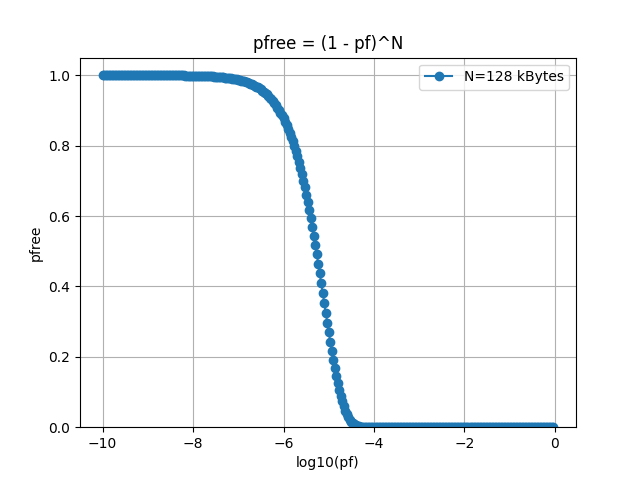
\includegraphics[width=0.90\linewidth]{Chapter-2/figs/pfree.png}
  \caption{Proportional \texttt{.text} and \texttt{.data} sizes for selected Linux utilities, measured with the \texttt{size} tool. Most binaries devote the large majority of bytes to instructions, and data rarely exceeds a small share of the image.}
  \label{fig:pfree}
\end{figure}

Figure~\ref{fig:pfree} illustrates the relationship between the probability of cell failure 
$p_f$ and the probability of overall system survival $p_{\mathrm{free}}$ for a memory of 
128~kBytes. The x-axis is shown on a logarithmic scale to highlight how rapidly the reliability 
collapses as $p_f$ increases.

When $p_f$ is extremely small (e.g., $10^{-10}$ or lower), the curve is flat and 
$p_{\mathrm{free}} \approx 1$, meaning that the system is almost always fault-free. However, 
as $p_f$ increases above $10^{-8}$, the probability of survival begins to decrease dramatically. 
This transition region is quite narrow: between $10^{-7}$ and $10^{-5}$ the survival 
probability drops from near certainty to almost zero. Once $p_f$ approaches $10^{-4}$, 
the probability of a fault-free system is negligible.

This steep ``S-curve'' behavior is a direct consequence of the exponential term 
$(1 - p_f)^N$. Although $p_f$ may still appear to be very small in absolute terms, 
the large value of $N$ (the total number of memory cells in 128~kBytes) amplifies the 
effect. The result is that the system-level reliability rapidly collapses as soon as 
the per-cell fault probability leaves the ultra-low range.

This figure demonstrates the central challenge of memory reliability: the difference 
between practically perfect yield and catastrophic unreliability may be within only a 
few orders of magnitude of $p_f$. It also motivates the use of replication, repair, or 
other fault-tolerant mechanisms to extend reliability when $p_f$ is not vanishingly small.

\section{Raw Error Rates vs. Unrecoverable Error Rates}
\label{sec:error-rates}

The discussion so far has focused on the \emph{raw error rate}, where $p_f$ represents 
the probability of a single cell experiencing a fault. This raw bit error rate has been 
reported to span a wide range in practice, from as low as $10^{-14}$ in highly reliable 
technology nodes up to $10^{-2}$ in more aggressive or degraded processes. As 
demonstrated in Figure~\ref{fig:pfree}, even small increases in $p_f$ can cause the 
system-level survival probability to collapse rapidly once the memory size is large.

However, raw error rate alone does not determine system reliability. In real systems, 
hardware and software employ a variety of techniques---such as error-correcting codes 
(ECC), block replacement, and redundancy---to detect and repair many of these raw 
faults before they propagate to execution. The rate that remains after all correction 
mechanisms is referred to as the \emph{unrecoverable error rate} (UER). This represents 
the fraction of faults that ultimately escape detection or exceed the correction 
capability of the system, and therefore pose a direct threat to correctness.

The gap between raw error rate and unrecoverable error rate is a measure of the 
effectiveness of the protection scheme. A strong ECC, for example, can tolerate many 
single-bit and some multi-bit upsets, driving the effective UER several orders of 
magnitude below the raw bit failure probability $p_f$. In contrast, in systems with 
little or no protection, the raw error rate and the unrecoverable error rate are nearly 
identical. 

This distinction is critical: The raw error rate gives a technology-level view of reliability, 
but the unrecoverable error rate determines whether the program will run correctly. 
The gap between the two depends on the effectiveness of protection mechanisms such as ECC, 
which is itself a design choice made by the system architect. A stronger ECC scheme 
reduces the unrecoverable error rate at the cost of additional area, power, and latency, 
while weaker or absent ECC leaves the system more exposed. In the following sections, 
we build on this by analyzing reliability at the function and program level under the 
assumption of persistent static memory faults.

\section{Limit Study}
\label{sec:ch2-limit-study}

\subsection{Overview}
\label{subsec:limit-overview}

Figure~\ref{fig:baseline-reliability} presents the results of the baseline limit study across several benchmarks. 
In this experiment, the per-bit fault probability was fixed at its maximum ($p_f = 1$). 
Instead of varying $p_f$, the fault injection rate $R$ was varied, where $R$ represents 
the average interval between injected faults, expressed in bytes. 
Smaller values of $R$ correspond to denser corruption, while larger values of $R$ correspond to sparser faults.  

To model this process statistically, the number of corrupted bytes within a memory block 
of size $M$ is represented by a Poisson random variable $N$ with mean $M / R$:

\begin{equation}
N \sim \mathrm{Poisson}\left(\frac{M}{R}\right)
\end{equation}

Each corrupted byte’s position $x_i$ is sampled independently from a uniform distribution 
over the block address space:

\begin{equation}
x_i \sim \mathrm{Uniform}\left(0,\; \left(\frac{M}{R}+1\right)M \right), \quad i = 1, \ldots, N
\end{equation}

Together, these relationships define the combined stochastic model:

\begin{equation}
N,\, x_i \sim 
\begin{cases}
N \sim \mathrm{Poisson}\left(\frac{M}{R}\right),\\[4pt]
x_i \sim \mathrm{Uniform}\left(0,\; \left(\frac{M}{R}+1\right)M \right)
\end{cases}
\label{cha2-eq-model}
\end{equation}

This model captures both the random number and spatial distribution of faults, 
providing a more accurate representation of fault behavior than deterministic expectations.

\subsection{Setup}
\label{subsec:baseline-setup}

The baseline limit study evaluates how system reliability degrades as the density of injected faults 
increases across a set of benchmark applications. 
The experimental workflow is shown in Figure~\ref{fig:fault-injection-flow}.  

Each benchmark executable (e.g., \texttt{bh}, \texttt{crc32}, and others) is processed 
through the fault injection function $I(R)$, which applies faults following the 
Poisson--Uniform model of Equation~\ref{cha2-eq-model}. 
Bits at those locations are flipped to create corrupted binaries.  

To maintain consistency across studies, fault injection is limited to a defined subset of 
non-library functions within each benchmark. Library routines remain unmodified because they 
are precompiled and shared with later experiments.  

Each corrupted executable is executed, and its output is compared to the fault-free 
reference output. Matching outputs indicate successful execution; mismatches or crashes 
are classified as failures.  

To capture statistical variation, the process is repeated $P$ times for each rate $R$. 
The resulting success fraction represents the empirical reliability of the baseline system.

\begin{figure}[t]
  \centering
  
\includegraphics[width=0.90\linewidth]{Chapter-2/figs/fault-injection-flow.png}
  \caption{Fault injection and evaluation flow for the baseline and FLCR studies. 
  Benchmarks are compiled and processed through the fault-injection function $I(R)$, 
  which introduces faults according to the Poisson–Uniform model. 
  Only non-library functions are targeted, and the process is repeated $P$ times per rate $R$.}
  \label{fig:fault-injection-flow}
\end{figure}

\subsection{Results}
\label{subsec:limit-results}

When the expected number of corrupted bytes per block ($M/R$) is much less than one, 
programs almost always execute correctly. As this expectation approaches one, reliability 
collapses sharply, and successful runs fall to near zero. 
This rapid transition highlights the exponential sensitivity of reliability to fault density.  

Although this pattern is consistent across all benchmarks, the exact point of collapse 
varies by application. Workloads such as \texttt{bh} and \texttt{crc32} fail earlier 
(higher $R$, lower corruption), while \texttt{rawcaudio} and \texttt{patricia} 
remain functional under denser faults.  

Overall, reliability remains high while $M / R < 1$ but declines precipitously 
once this threshold is exceeded.

\begin{figure}[t]
  \centering
  
\includegraphics[width=0.90\linewidth]{Chapter-2/figs/baseline-reliability.png}
  \caption{Baseline limit study results across benchmarks. 
  The x-axis shows the fault rate $\log_{10}(1/R)$; the y-axis shows the number of successful permutations. 
  Reliability collapses once the expected number of corrupted bytes per block approaches one.}
  \label{fig:baseline-reliability}
\end{figure}

\section{Beyond Hardware ECC Protection}
\label{sec:beyond-ecc}

Error-Correcting Codes (ECC) are the most widely deployed hardware mechanism for 
protecting memory reliability. Typical systems use schemes such as single-error 
correction and double-error detection (SECDED), while higher-reliability systems 
may employ stronger codes. These approaches substantially reduce the unrecoverable 
error rate by masking or repairing most single-bit upsets and detecting many 
double-bit errors. The effectiveness of ECC is a design choice made by the system 
architect, trading off correction strength against cost in area, power, latency, 
and memory overhead.  

Despite its value, hardware ECC has inherent limits. Every ECC scheme can only correct 
a bounded number of errors within a block. Once this threshold is exceeded, additional 
errors become unrecoverable. The limit study in Figure~\ref{fig:baseline-reliability} 
illustrates this point: reliability collapses sharply once the expected number of 
faulty bytes per block approaches one, regardless of how small the raw bit error rate 
may be. No practical ECC can fully prevent this collapse, since codes are always 
dimensioned with finite correction capacity.  

Once ECC reaches its correction limit, it can quickly become unreliable, since any 
additional errors often render the entire protected block unusable. Rather than attempting 
to increase the strength of ECC---which adds significant hardware overhead---a 
complementary software solution can be used to improve reliability.  
